\documentclass[12pt,a4paper]{article}
\usepackage{amsmath,amscd,amsbsy,amssymb,latexsym,url,bm,amsthm}
\usepackage{epsfig,graphicx,subfigure}
\usepackage{enumitem,balance}
\usepackage{wrapfig}
\usepackage{mathrsfs, euscript}
\usepackage[usenames]{xcolor}
\usepackage{hyperref}
\usepackage[vlined,ruled,commentsnumbered,linesnumbered]{algorithm2e}
\usepackage{float}
\usepackage{array}
\usepackage{diagbox}
\usepackage{color}
\usepackage{indentfirst}
\usepackage{fancyhdr}
\usepackage{gensymb}
\usepackage{geometry}
\usepackage{setspace}
\usepackage{aurical}
\usepackage{times}
\usepackage{caption}
\usepackage{fontspec}
\usepackage{booktabs}
\setmainfont{Times New Roman}

\newtheorem{theorem}{Theorem}[section]
\newtheorem{lemma}[theorem]{Lemma}
\newtheorem{proposition}[theorem]{Proposition}
\newtheorem{corollary}[theorem]{Corollary}
\newtheorem{exercise}{Exercise}[section]
\newtheorem*{solution}{Solution}
\theoremstyle{definition}

\newcommand{\postscript}[2]
 {\setlength{\epsfxsize}{#2\hsize}
  \centerline{\epsfbox{#1}}}
\renewcommand{\baselinestretch}{1.0}

\setlength{\oddsidemargin}{-0.365in}
\setlength{\evensidemargin}{-0.365in}
\setlength{\topmargin}{-0.3in}
\setlength{\headheight}{0in}
\setlength{\headsep}{0in}
\setlength{\textheight}{10.1in}
\setlength{\textwidth}{7in}
\makeatletter \renewenvironment{proof}[1][Proof] {\par\pushQED{\qed}\normalfont\topsep6\p@\@plus6\p@\relax\trivlist\item[\hskip\labelsep\bfseries#1\@addpunct{.}]\ignorespaces}{\popQED\endtrivlist\@endpefalse} \makeatother
\makeatletter
\renewenvironment{solution}[1][Solution] {\par\pushQED{\qed}\normalfont\topsep6\p@\@plus6\p@\relax\trivlist\item[\hskip\labelsep\bfseries#1\@addpunct{.}]\ignorespaces}{\popQED\endtrivlist\@endpefalse} \makeatother

\begin{document}
\noindent
%==========================================================
\noindent\framebox[\linewidth]{\shortstack[c]{
\Large{\textbf{Report on Homework 3 -- SVM vs. Neural Networks}}\vspace{1mm}\\ 
CS420, Machine Learning, Shikui Tu, Summer 2018 \vspace{1mm} \\
Zelin Ye 515030910468}}

\section{Introduction}

In machine learning, SVM (Support Vector Machine) is a commonly used classfication method due to its high efficiency and accuracy. Recent years, the neural network has been attracting more and more attention, and also used to solve classification problems. In this homework, I would investigate the performances of SVM and neural network (e.g. MLP) on some classification datasets under different experimental settings (e.g. pass).

\section{Methodology}

In this section, I would introduce the datasets and models in my experiments.

\subsection{Datasets}

In my experiments, I use two datasets that are from \textbf{LIBSVM Data} \cite{dataA} to investigate the performances of SVM and neural network. One is \textbf{splice} \cite{splice}, a binary classification dataset with 60 features, 1000 training samples and 2175 testing samples. Another is called \textbf{satimage} \cite{satimage}, which is for multi-class classification and has 36 features, 6 classes, 3104 training samples and 2000 testing samples.

Additionally, I choose a dataset called \textbf{CIFAR-10} \cite{cifar-10} from LISA \cite{dataB} to conduct comparison between SVM and deep learning algorithm benchmarks. It is a multi-class classification dataset that contains 10 classes, $32 \times 32 \times 3 = 3072$ features, 50000 training samples (divided equally into 5 batches) and 10000 testing samples.

More details about these datasets can refer to Appendix \ref{apd:dataset}.

\subsection{Models}

For neural network, considering the complexity of features and scale of samples, I choose MLP (Multi-layer Perceptron) instead of popular DNN or CNN.

\vspace{0.01\linewidth}
In experiments, I would investigate the performances of MLP under different architectures or parameter settings (e.g. number of hidden layers or hidden neurons).

\section{Experiments and Results}

\subsection{Preprocess}

Most datasets are likely to have missing data, and those in LIBSVM Data are no exception. Therefore, I first make up for the omission in the datasets, replacing empty data with corresponding mean values. Afterwards, I convert the labels from numbers to one-hot vectors for the calculation of loss.

\subsection{SVM}
\label{sec:svm}

In this section, I would show the performances of SVM in both \textit{splice} and \textit{satimage} datasets under different configurations (e.g. pass). Note that the two datasets have different problem settings, sample sizes and etc. I would thus conduct some pertinent discussion based on each experiment result.

\vspace{0.01\linewidth}
Without special explanation, except for the target parameter, the experiments are based on default parameters of \textit{sklearn} \cite{sklearn} (a Python package for machine learning), which can refer to Tab. \ref{tab:default-para}.

\begin{table}[H]
	\renewcommand\arraystretch{1.35}
	\caption{Some important default parameters of SVM experiments}
	\label{tab:default-para}
	\centering
	
	\begin{tabular}{c|c|c}
		\centering
		Name & Meaning & Value \\
		\hline
		\hline
		
		C & penalty parameter of the error term & 1.0 \\
		degree & degree of the polynomial kernel function & 3 \\
		gamma & kernel coefficient for 'rbf', 'poly' and 'sigmoid' & 1/n\_features \\
		coef0 & independent term in kernel function & 0.0 \\
		shrinking & whether to use the shrinking heuristic & True \\
		tol & tolerance for stopping criterion & 1e-3 \\
		decision\_function\_shape & one-vs-rest or one-vs-one & ovr \\
		
	\end{tabular}
\end{table}

With these default parameters, I train a baseline model as a reference (Fig. \ref{fig:svm-baseline}). According to the normal principle, I should measure the performance with f1-score, but I tend to make the results more intuitive and I use the \textbf{accuracy} of classification as the criterion.

\begin{figure}[H]
	\centering
	\subfigure[Splice]{
		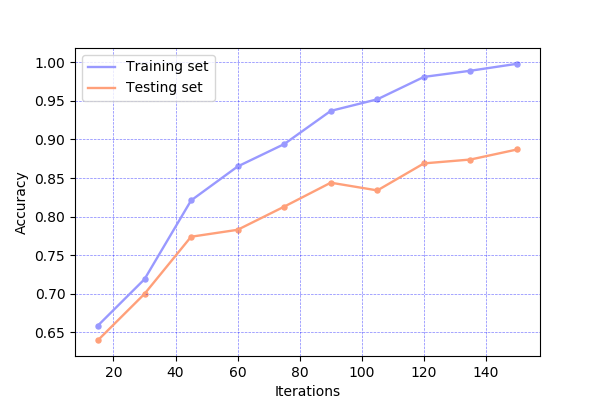
\includegraphics[width=0.45\linewidth]{img/svm_baseline_splice.png}
	}
	\subfigure[Satimage]{
		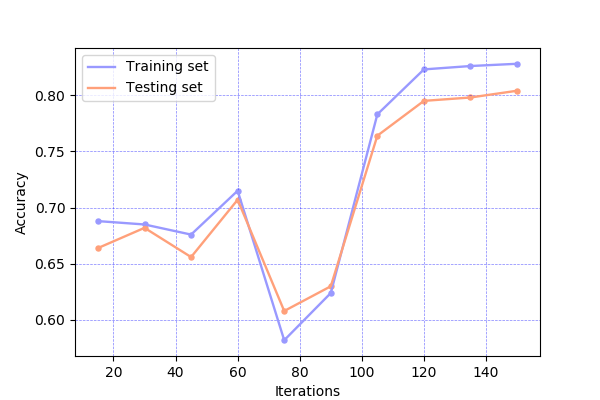
\includegraphics[width=0.45\linewidth]{img/svm_baseline_sat.png}
	}
	\caption{The baseline of SVM.}
	\label{fig:svm-baseline}
\end{figure}

\subsubsection{Kernel}

The ability of SVM might be constrainted when dealing with non-linear features, where kernel trick could resolve this issue. Nevertheless, a successful choice of kernel is still based on experience or luck. I apply several kernels to SVM and get the following results (Fig. \ref{fig:svm-kernel}).

\begin{figure}[H]
	\centering
	\subfigure[Splice-Training Set]{
		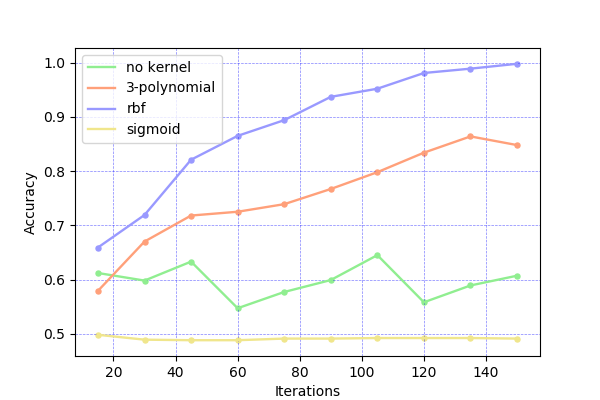
\includegraphics[width=0.45\linewidth]{img/svm_kernel_splice_tr.png}
	}
	\subfigure[Splice-Tetsing Set]{
		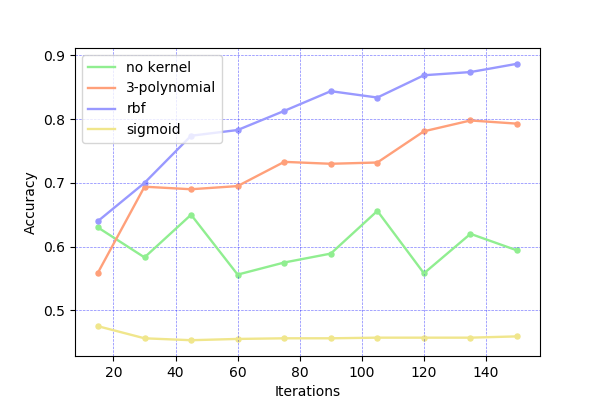
\includegraphics[width=0.45\linewidth]{img/svm_kernel_splice_t.png}
	}
	\subfigure[Satimage-Training Set]{
		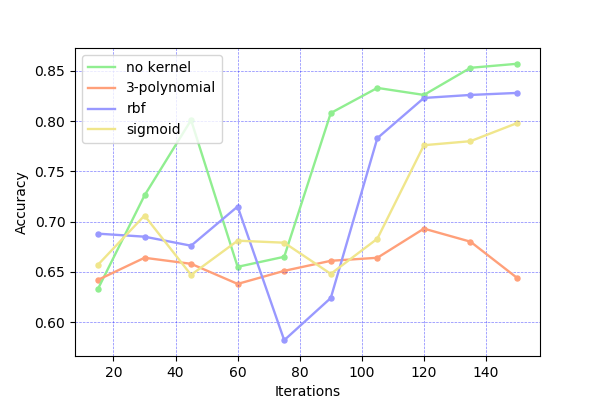
\includegraphics[width=0.45\linewidth]{img/svm_kernel_sat_tr.png}
	}
	\subfigure[Satimage-Testing Set]{
		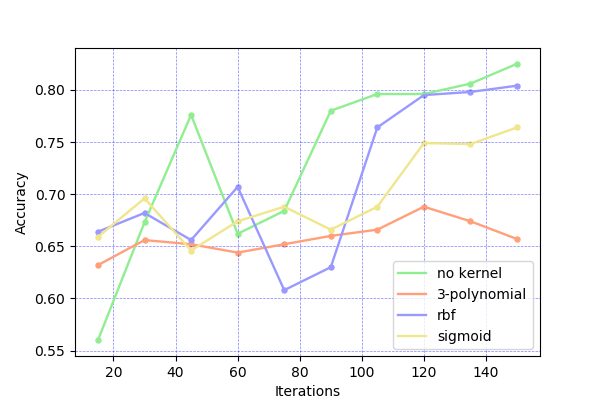
\includegraphics[width=0.45\linewidth]{img/svm_kernel_sat_t.png}
	}
	\caption{The performances of SVM under different kernels.}
	\label{fig:svm-kernel}
\end{figure}

It is apparent that the effect of these kernels differ greatly. Rbf (Radial Basis Function) kernel is most suitable for \textit{splice} while no kernel function is the best choice for \textit{satimage}. 

\vspace{0.01\linewidth}
Additionally, the selection of specific parameters of a kernel would also affect the results. I test polynomial kernel with different degrees, the test error can refer to Tab. \ref{tab:kernel-poly}.

\begin{table}[H]
	\renewcommand\arraystretch{1.35}
	\caption{The performances of polynomial kernel under different degrees}
	\label{tab:kernel-poly}
	\centering
	
	\begin{tabular}{c|c|c}
		\centering
		Degree & Test Error (Splice) & Test Error (Satimage) \\
		\hline
		
		2 & 0.786 & 0.635 \\
		3 & 0.857 & 0.666 \\
		4 & 0.865 & 0.505 \\
		5 & 0.871 & 0.554 \\
		6 & 0.880 & 0.488 \\
		7 & 0.874 & 0.512 \\
		8 & 0.864 & 0.477 \\
		9 & 0.867 & 0.528 \\
		10 & 0.851 & 0.403 \\
	\end{tabular}
\end{table}

The trend reflected in the table is that higher degree can reduce training error, but lead to more test error in the meantime. Still, the performance would also drop a lot in both training set and test set when the degree is too large. This result also proves the significance fo choosing the complexity of model properly.

\subsubsection{Penalty Parameter}

Although SVM would encounter difficulties on non-linear data, it can still handle slightly non-separable data via soft-margin technique (transforming the optimization object into $\dfrac{1}{2}w^Tw+C\sum\limits_{n=1}^{N}\xi_n$), where the penalty parameter $C$ is critical for classification performance. I have tried the $C$ of different orders of magnitude, and the results can be found in Fig. \ref{fig:svm-penalty}.

\begin{figure}[H]
	\centering
	\subfigure[Splice]{
		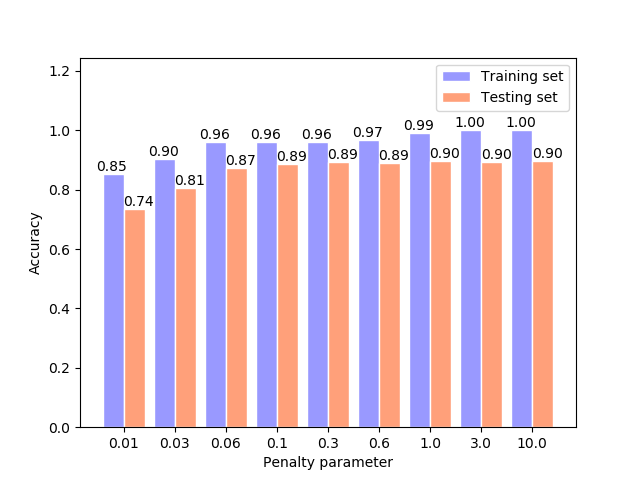
\includegraphics[width=0.45\linewidth]{img/svm_penalty_splice.png}
	}
	\subfigure[Satimage]{
		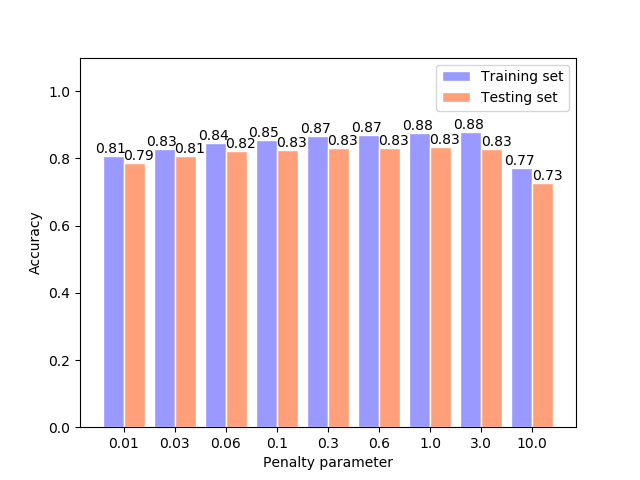
\includegraphics[width=0.45\linewidth]{img/svm_penalty_sat.png}
	}
	\caption{The performances of SVM under different penalty parameter $C$.}
	\label{fig:svm-penalty}
\end{figure}

According to the results, the introduction of $C$ is sometimes beneficial to the classification. More specifically, proper $C$ could improve the performance of SVM while excessive $C$ might produce additional errors. In general, the circumstances might vary a little bit according to the data, where $C$ should be determined by large scale of experiments.

\subsubsection{Dimension of Features}



\begin{figure}[H]
	\centering
	\subfigure[Splice-Training Set]{
		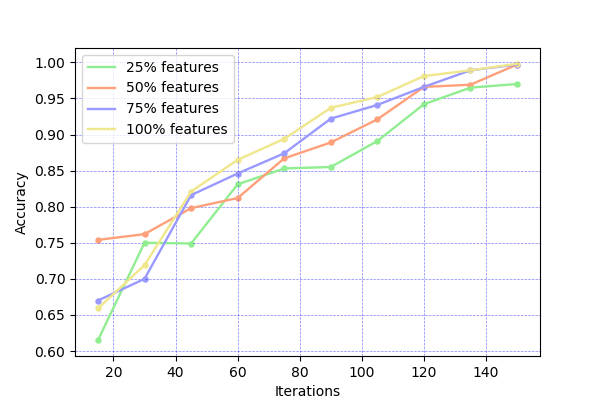
\includegraphics[width=0.45\linewidth]{img/svm_dim_splice_tr.png}
	}
	\subfigure[Splice-Tetsing Set]{
		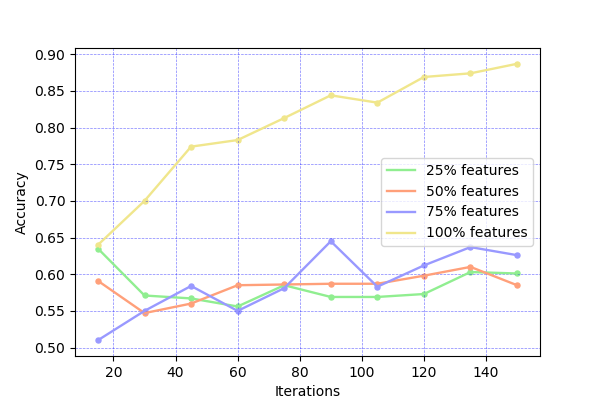
\includegraphics[width=0.45\linewidth]{img/svm_dim_splice_t.png}
	}
	\subfigure[Satimage-Training Set]{
		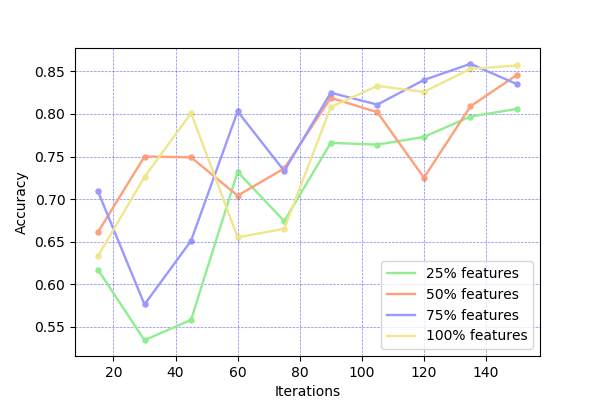
\includegraphics[width=0.45\linewidth]{img/svm_dim_sat_tr.png}
	}
	\subfigure[Satimage-Testing Set]{
		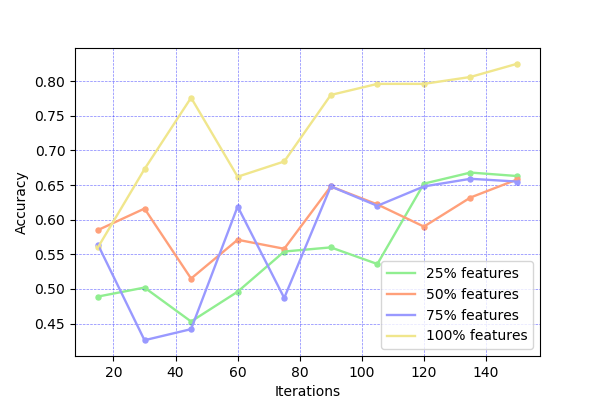
\includegraphics[width=0.45\linewidth]{img/svm_dim_sat_t.png}
	}
	\caption{The performances of SVM under different dimensions of features.}
	\label{fig:svm-dim}
\end{figure}

\subsubsection{Summarization}

SVM is a powerful tool for classification, which can achieve satisfactory results in both binary and multi-class classification problems. Meanwhile, SVM could take advantage of many tricks (e.g. soft-margin, kernel) to extend its application scope and improve its performance. If SVM is applied to small scale problems with appropriate configurations, it would perform quite well.

\subsection{Neural Network}

In this section, I would also show the performances of MLP in the two datasets under different configurations (e.g. optimization algorithms, network architectures). In the meantime, I would also analyze each result concisely.

\vspace{0.01\linewidth}
Same as Sec. \ref{sec:svm}, I conduct the following experiments based on default parameters in \textit{sklearn}. Some important parameters are shown in Tab. \ref{tab:default-para-mlp} and the baseline model can refer to Fig. \ref{fig:mlp-baseline}.

\begin{table}[H]
	\renewcommand\arraystretch{1.35}
	\caption{Some important default parameters of MLP experiments}
	\label{tab:default-para-mlp}
	\centering
	
	\begin{tabular}{c|c|c}
		\centering
		Name & Meaning & Value \\
		\hline
		\hline
		
		hidden\_layer\_sizes & the size of hidden layers & (100,) \\
		activation & activation function for the hidden layer & relu \\
		solver & the solver for weight optimization & adam \\
		alpha & L2 penalty (regularization term) parameter & 0.0001 \\
		batch\_size & size of minibatches for stochastic optimizers & min(200, n\_samples) \\
		learning\_rate\_init & the initial learning rate used & 0.001 \\
		power\_t & the exponent for inverse scaling learning rate & 0.5 \\
		tol & tolerance for the optimization & 1e-4 \\
		
	\end{tabular}
\end{table}

\begin{figure}[H]
	\centering
	\subfigure[Splice]{
		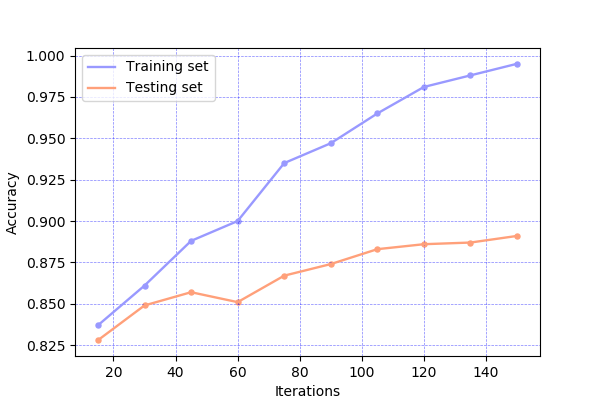
\includegraphics[width=0.45\linewidth]{img/mlp_baseline_splice.png}
	}
	\subfigure[Satimage]{
		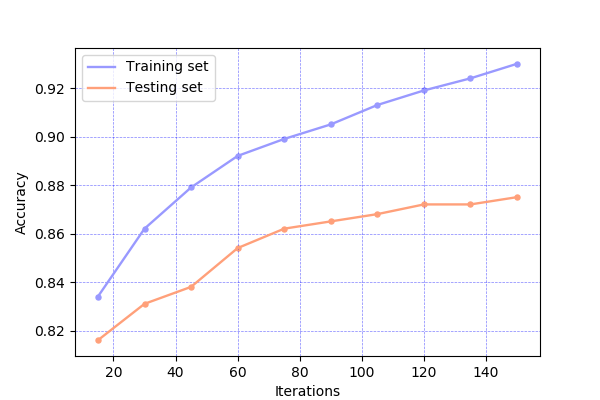
\includegraphics[width=0.45\linewidth]{img/mlp_baseline_sat.png}
	}
	\caption{The baseline of MLP.}
	\label{fig:mlp-baseline}
\end{figure}

\subsubsection{Optimization Algorithm}
\label{sec:optim}

Optimization algorithms refer to a series algorithms used to update parameters of neural network (e.g. sgd, adam \cite{adam}). The optimal direction and effect of these algorithms are quite different, Fig. \ref{fig:example} is a visual illustration.

\begin{figure}[H]
	\centering
	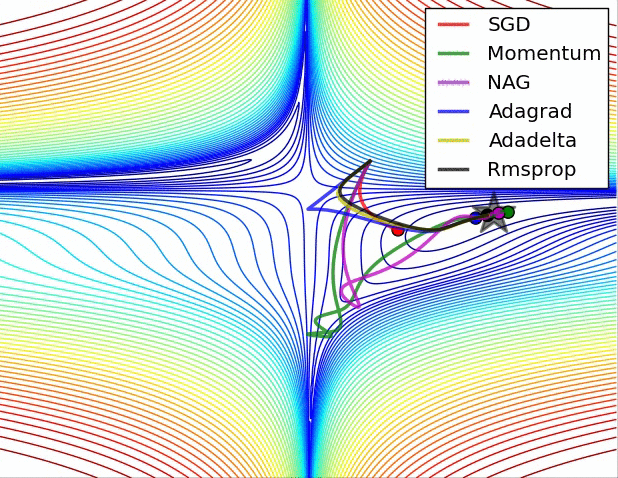
\includegraphics[width=0.45\linewidth]{img/optim_example.png}
	\caption{The visual illustration of optimization algorithms \cite{optim_example}.}
	\label{fig:example}
\end{figure}

Since the performance of MLP is greatly influenced by the optimization algorithms, I tend to investigate it in detail. I test the effect of three typical algorithms: \textbf{lbfgs}, \textbf{sgd} and \textbf{adam}. The corresponding training processes are shown in Fig. \ref{fig:mlp-optimizer}.

\begin{figure}[H]
	\centering
	\subfigure[Splice-Training Set]{
		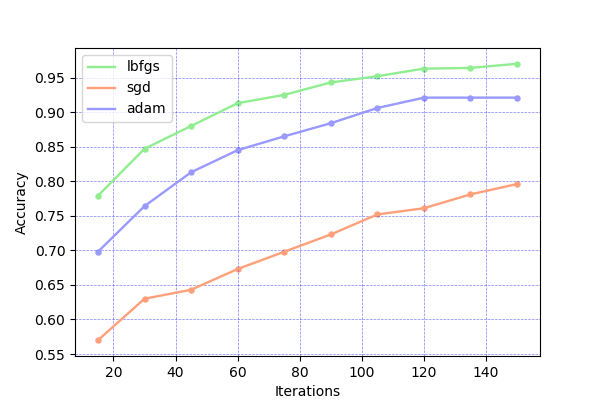
\includegraphics[width=0.45\linewidth]{img/mlp_optimizer_splice_tr.png}
	}
	\subfigure[Splice-Tetsing Set]{
		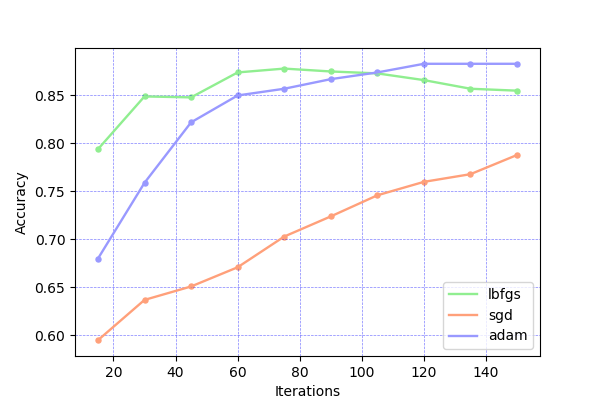
\includegraphics[width=0.45\linewidth]{img/mlp_optimizer_splice_t.png}
	}
	\subfigure[Satimage-Training Set]{
		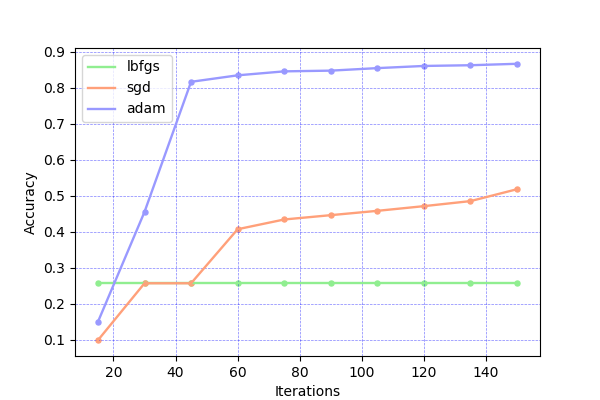
\includegraphics[width=0.45\linewidth]{img/mlp_optimizer_sat_tr.png}
	}
	\subfigure[Satimage-Testing Set]{
		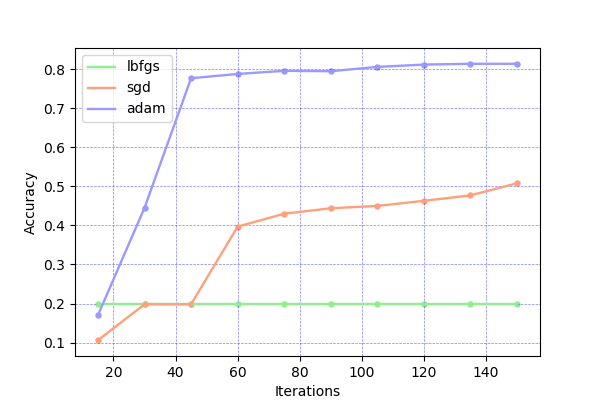
\includegraphics[width=0.45\linewidth]{img/mlp_optimizer_sat_t.png}
	}
	\caption{The performances of MLP under different optimization algorithms.}
	\label{fig:mlp-optimizer}
\end{figure}

The results in two datasets are consistent with the theoretical analysis: the effect of optimization algorithms differ awfully. It seems that \textit{adam} achieves the best effect in both datasets (though \textit{lbfgs} has lower training error, it might encounter overfitting in \textit{splice}). In \textit{satimage}, the rest two algorithms have poor performance, \textit{lbfgs} even falls into the local minimum at the beginning of training.

\vspace{0.01\linewidth}
In brief, \textit{adam} algorithm could achieve satisfactory results in most cases, the optimization effect of \textit{sgd} is weaker and \textit{lbfgs} might be instable.

\subsubsection{Activation Function}

Activation function is an indispensable component of MLP. It extends the scope MLP can represent with introducing non-linear factors into MLP. I compare the effects of 3 commonly used activation functions (\textbf{relu} \cite{relu}, \textbf{sigmoid} and \textbf{tanh}) on two datasets (Fig. \ref{fig:mlp-activation}).

\begin{figure}[H]
	\centering
	\subfigure[Splice-Training Set]{
		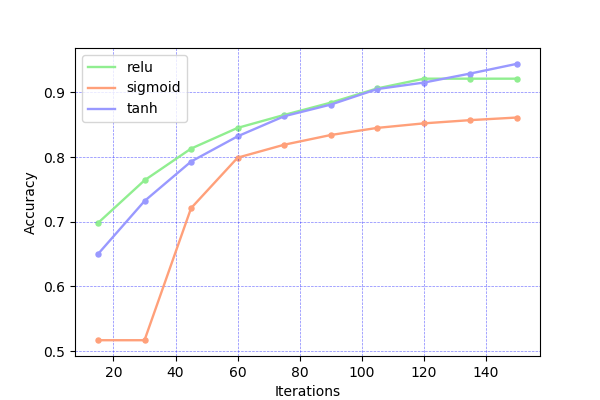
\includegraphics[width=0.45\linewidth]{img/mlp_activation_splice_tr.png}
	}
	\subfigure[Splice-Tetsing Set]{
		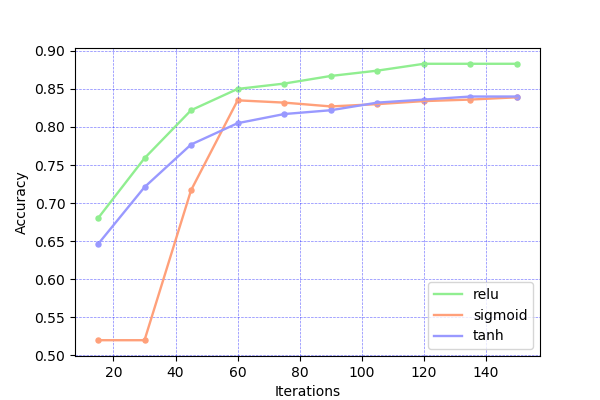
\includegraphics[width=0.45\linewidth]{img/mlp_activation_splice_t.png}
	}
	\subfigure[Satimage-Training Set]{
		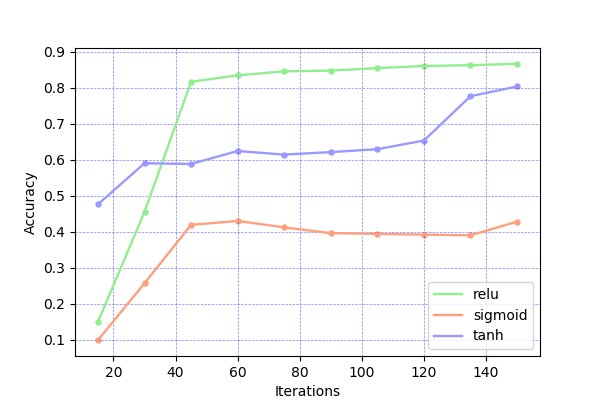
\includegraphics[width=0.45\linewidth]{img/mlp_activation_sat_tr.png}
	}
	\subfigure[Satimage-Testing Set]{
		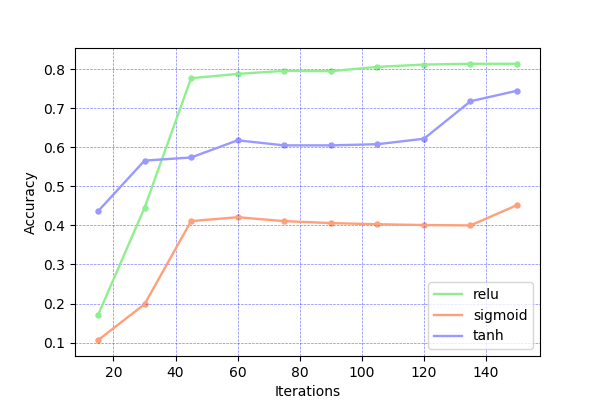
\includegraphics[width=0.45\linewidth]{img/mlp_activation_sat_t.png}
	}
	\caption{The performances of MLP under different activation functions.}
	\label{fig:mlp-activation}
\end{figure}

Similar to Sec. \ref{sec:optim}, the effects of different activation function are widely divergent, especially on \textit{satimage}. In most cases, \textit{relu} is undoubtedly the best choice. \textit{sigmoid} and \textit{tanh} could be applied to simple problems, their effects will be greatly reduced when confronted with complex problems.

\subsubsection{Learning Rate}

In training process, learning rate controls the speed of updating parameters. Researchers often pours quantities of time into adjusting learning rate due to its large effect to training results. I investigate the classification results on several orders of magnitude of learning rate (Fig. \ref{fig:mlp-lr}).

\begin{figure}[H]
	\centering
	\subfigure[Splice]{
		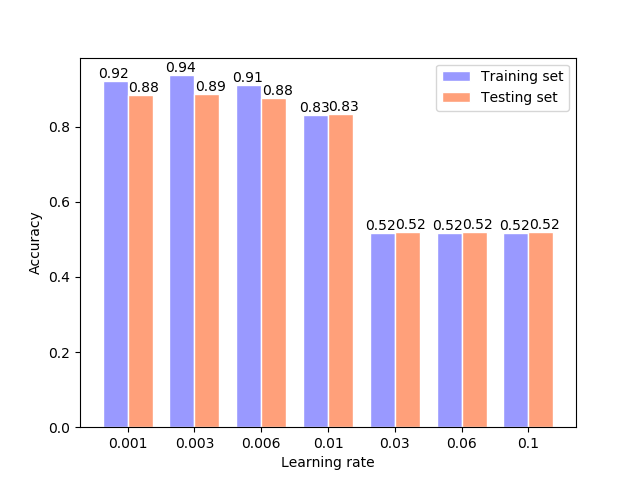
\includegraphics[width=0.45\linewidth]{img/mlp_lr_splice.png}
	}
	\subfigure[Satimage]{
		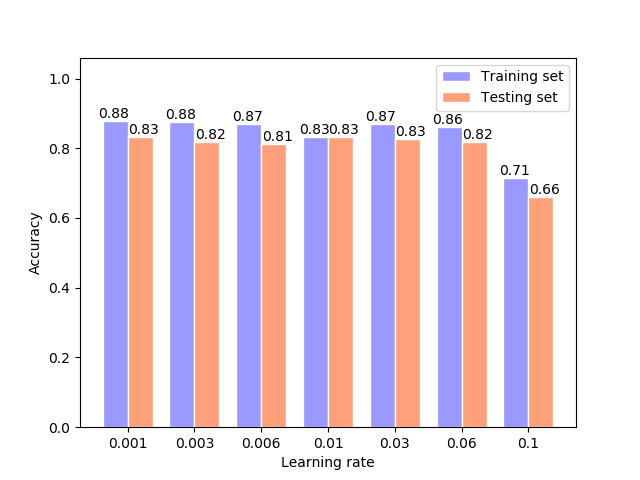
\includegraphics[width=0.45\linewidth]{img/mlp_lr_sat.png}
	}
	\caption{The performances of MLP under different learning rate.}
	\label{fig:mlp-lr}
\end{figure}

According to above results, learning rates of 0.003 and 0.001 could provide best performance for MLP on \textit{splice} and \textit{satimage} respectively. Unfortunately, even the best results in Fig. \ref{fig:mlp-lr} have no improvement compared with baseline (Fig. \ref{fig:mlp-baseline}), this also illustrates the difficulty of learning rate adjustment.

\subsubsection{Network Architecture}

In addition to the above configuration factors, the network architecture of MLP also contributes a lot to final results. There are two simple changes to the network architecture: deepening the network and increasing the number of nuerons of each layer. I have tried several architectures based on these two changes (Fig. \ref{fig:mlp-archi}).

\begin{figure}[H]
	\centering
	\subfigure[Splice-Training Set]{
		\label{fig:mlp-archi-a}
		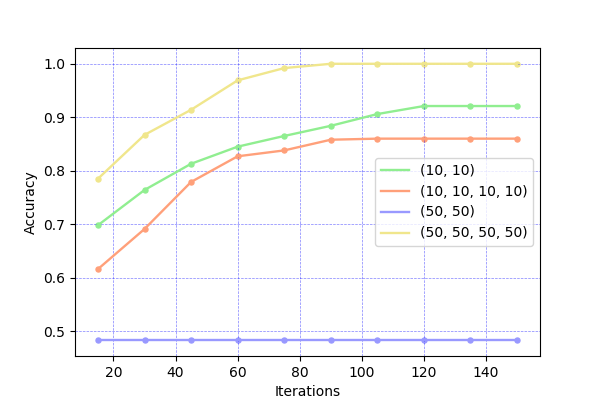
\includegraphics[width=0.45\linewidth]{img/mlp_archi_splice_tr.png}
	}
	\subfigure[Splice-Tetsing Set]{
		\label{fig:mlp-archi-b}
		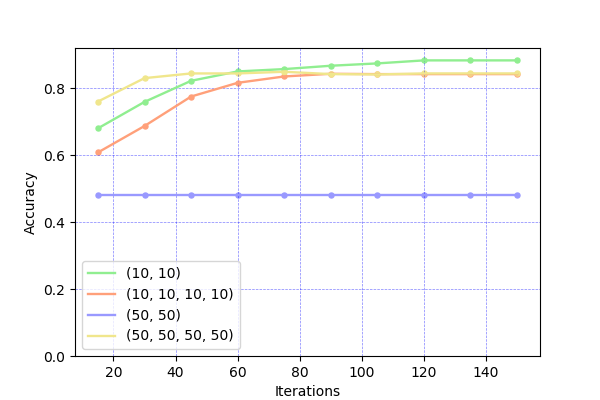
\includegraphics[width=0.45\linewidth]{img/mlp_archi_splice_t.png}
	}
	\subfigure[Satimage-Training Set]{
		\label{fig:mlp-archi-c}
		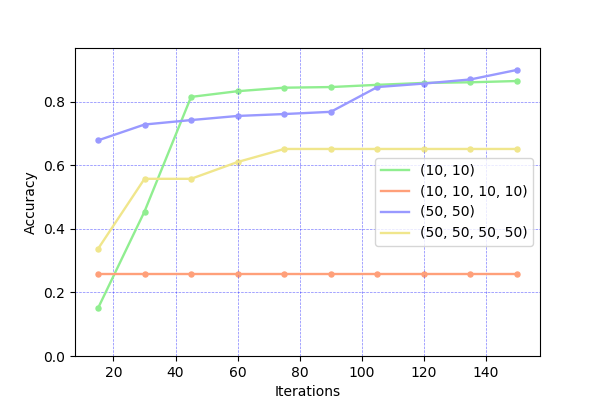
\includegraphics[width=0.45\linewidth]{img/mlp_archi_sat_tr.png}
	}
	\subfigure[Satimage-Testing Set]{
		\label{fig:mlp-archi-d}
		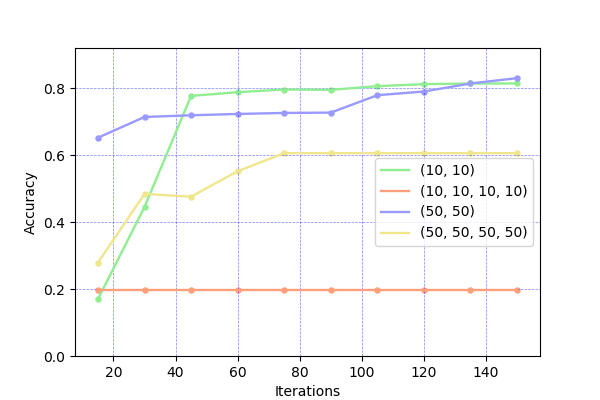
\includegraphics[width=0.45\linewidth]{img/mlp_archi_sat_t.png}
	}
	\caption{The performances of MLP under different network architectures (the numbers in brackets indicate the number of neurons in each layer).}
	\label{fig:mlp-archi}
\end{figure}

For a certain dataset, appropriate architectures would be propitious to good performance, like red and yellow lines in Fig. \ref{fig:mlp-archi-b} and yellow line in Fig. \ref{fig:mlp-archi-d}. Otherwise, unsuitable architectures might crash the whole training process (blue line in Fig. \ref{fig:mlp-archi-b} and red line in Fig. \ref{fig:mlp-archi-d}).

\subsubsection{Dimension of Features}

\begin{figure}[H]
	\centering
	\subfigure[Splice-Training Set]{
		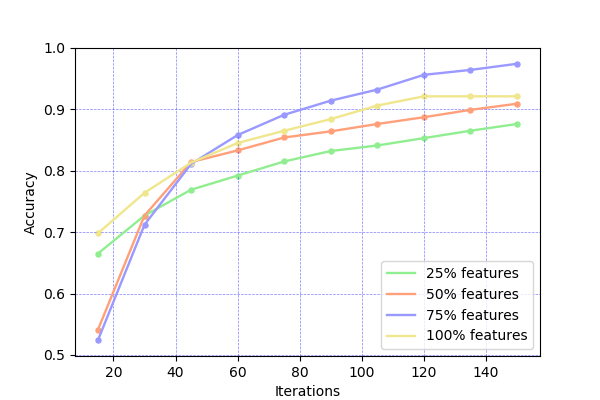
\includegraphics[width=0.45\linewidth]{img/mlp_dim_splice_tr.png}
	}
	\subfigure[Splice-Tetsing Set]{
		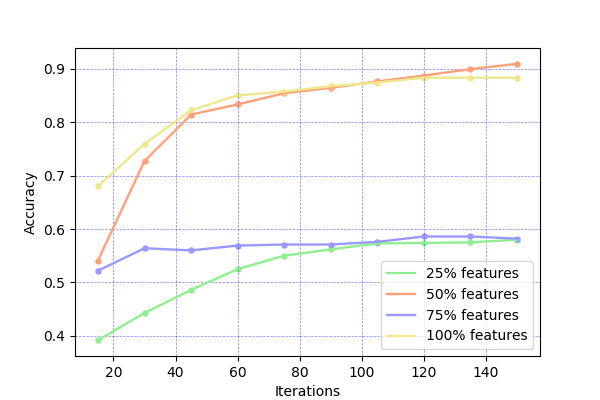
\includegraphics[width=0.45\linewidth]{img/mlp_dim_splice_t.png}
	}
	\subfigure[Satimage-Training Set]{
		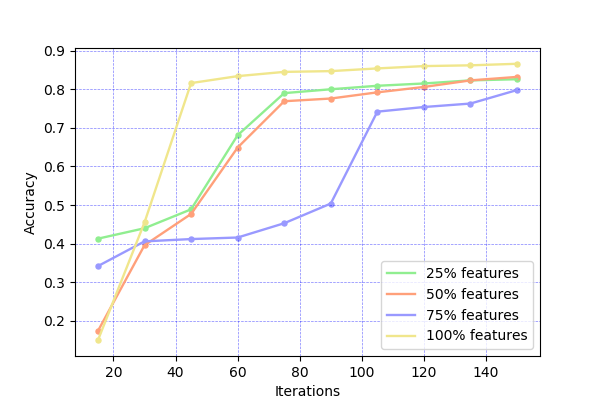
\includegraphics[width=0.45\linewidth]{img/mlp_dim_sat_tr.png}
	}
	\subfigure[Satimage-Testing Set]{
		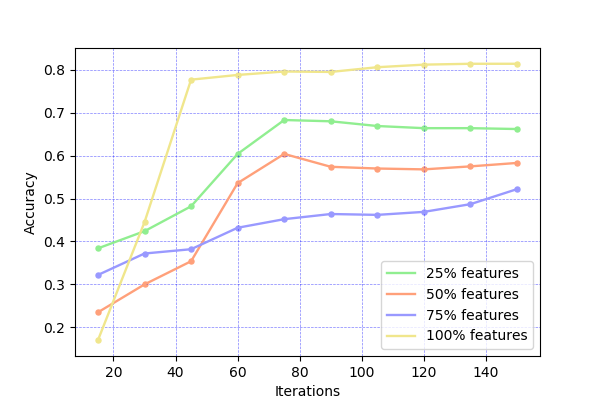
\includegraphics[width=0.45\linewidth]{img/mlp_dim_sat_t.png}
	}
	\caption{The performances of MLP under different dimensions of features.}
	\label{fig:mlp-dim}
\end{figure}

\subsubsection{Summarization}
\label{sec:sum-mlp}

MLP is a common way for a variety of problems. It owns a broader representation ability and stability compared with SVM and the baselines (Fig. \ref{fig:svm-baseline} and Fig. \ref{fig:mlp-baseline}) also prove this. Still, an available MLP model often takes much time to finetune, even a small change on any one component might make a great difference.

\section{Comparison Between SVM and Deep Learning Algorithm Benchmark}

In this section, I would show the application of SVM on CIFAR-10 dataset \cite{cifar-10} and compare the results to \href{https://code.google.com/archive/p/cuda-convnet/}{corresponding deep learning algorithm benchmark}. These results were obtained with a convolutional neural network. Briefly, the best of them is 18\% test error without data augmentation and 11\% with.

\subsection{Baseline of SVM}
\vspace{0.01\linewidth}
I first try SVM with default parameters of \textit{sklearn} on CIFAR-10 and get a terrible result: 0.123 training error and 0.105 test error for about 6 minutes on INTEL I5-5200U. I infer that such result might be out of the high dimension of features and large scale of samples. Then I start to adjust the SVM to improve the baseline performance.

\subsection{Finetune}
\label{sec:finetune}

\paragraph{1. Kernel}

\vspace{0.01\linewidth}
Since the performance of SVM on CIFAR-10 is pretty poor, I think it is difficult to improving this just by adjusting numerical parameters. Therefore, I start with picking out the most appropriate kernel.

\vspace{0.01\linewidth}
I have tried 3 kinds of kernels on each batch of CIFAR-10 with 100 iterations (more iterations does not make any difference) and default parameters of \textit{sklearn}. The results can refer to Tab. \ref{tab:bonus-kernel}.

\begin{table}[H]
	\renewcommand\arraystretch{1.35}
	\caption{The performances of different kernels on CIFAR-10}
	\label{tab:bonus-kernel}
	\centering
	
	\begin{tabular}{c|c|c|c|c|c|c}
		\centering
		 & Batch 1 & Batch 2 & Batch 3 & Batch 4 & Batch 5 & All data \\
		\hline
		
		RBF (training error) & 0.193 & 0.192 & 0.196 & 0.192 & 0.198 &  0.123 \\
		RBF (test error) & 0.105 & 0.103 & 0.105 & 0.105 & 0.105 & 0.105 \\
		Polynomial (training error) & 0.223 & 0.236 & 0.245 & 0.248 & 0.244 & 0.170 \\
		Polynomial (test error) & 0.209 & 0.218 & 0.213 & 0.229 & 0.228 & 0.172 \\
		Sigmoid (training error) & 0.098 & 0.098 & & & &  \\
		Sigmoid (test error) & 0.100 & 0.100 & & & &  \\
	\end{tabular}
\end{table}

As is shown in the above table, kernel achieve best performance.

\paragraph{2. Parameters of xxx Kernel}

\paragraph{3. Penalty Parameter}

Ultimately, I focus on finetuning penalty parameter $C$.

\subsection{Strengths and Weaknesses of SVM on Big Datasets}

According to the results in Sec. \ref{sec:finetune}, SVM perform poorly on a big dataset CIFAR-10. Note that the so-called 'big dataset' here refer to those datasets with more than tens of thousands of samples or thousands of features. In combination with the theoretical and experimental results, I think the weaknesses of SVM on big datasets consist of the following aspects:

\begin{enumerate}
	\item 1
\end{enumerate}

\newpage
\begin{appendix}
\section{Appendix}

\subsection{Details of Datasets in Experiments}
\label{apd:dataset}

\subsubsection{Splice \cite{splice}}

Basically, according to the biological knowledge, splice junctions are points on a DNA sequence at which `superfluous' DNA is removed during the process of protein creation in higher organisms.

\vspace{0.01\linewidth}
Splice dataset aims to recognize two classes of splice junctions, given a DNA sequence, the boundaries between exons (the parts of the DNA sequence retained after splicing) and introns (the parts of the DNA sequence that are spliced out).

\subsubsection{Satimage \cite{satimage}}

Satimage dataset is also called \textbf{satalog} dataset. It contains multi-spectral values of pixels in 3 $\times$ 3 neighbourhoods in satellite images, and the classification associated with the central pixel in each neighbourhood.

\vspace{0.01\linewidth}
As a classification dataset, the aim of satimage is to predict the classification, given the multi-spectral values. In the sample database, the class of a pixel is coded as a number.

\subsubsection{CIFAR-10 \cite{cifar-10}}

The CIFAR-10 dataset is labeled subsets of the 80 million tiny images dataset, collected by Alex Krizhevsky, Vinod Nair, and Geoffrey Hinton. CIFAR-10 consists of 60000 $32 \times 32$ colour images (50000 for training (divided into 5 batches), 10000 for test) in 10 classes, with 6000 images per class.


\vspace{0.01\linewidth}
Note that the classes of CIFAR-10 are completely mutually exclusive and there is no overlap between two classes (e.g. automobiles and trucks).


\end{appendix}

\bibliographystyle{ieeetr}
\bibliography{bio}

\end{document}